\documentclass[12pt]{article}
\usepackage[utf8]{inputenc}
\usepackage{lineno}
\usepackage{authblk}
\usepackage[margin=1in]{geometry}
\usepackage{xparse}
\usepackage{xpunctuate}
\usepackage{xspace}
\usepackage{graphicx}
\usepackage{wrapfig}
\usepackage[hidelinks]{hyperref}
\usepackage[all]{hypcap}
\usepackage{amsmath}
\usepackage{cleveref}
\usepackage{placeins}
\usepackage{flafter}
\usepackage{floatrow}
\usepackage{minted} 
\usepackage{caption}
\usepackage{float}
\usepackage{csvsimple}
\usepackage{booktabs}
\usepackage{siunitx}
\usepackage{natbib}

% local definitions
\newcommand{\msprime}[0]{\texttt{msprime}\xspace}
\newcommand{\tskit}[0]{\texttt{tskit}\xspace}
\newcommand{\slim}[0]{\texttt{SLiM}\xspace}
\newcommand{\pyslim}[0]{\texttt{pyslim}\xspace}
\newcommand{\allel}[0]{\texttt{scikit-allel}\xspace}
\newcommand*{\eg}{e.g.\xcomma}
\newcommand*{\ie}{i.e.\xcomma}
\newcommand{\comment}[1]{\textit{\color{green} #1}}
\newcommand{\p}[1]{\texttt{p#1}}

% syntax highlighting
\usepackage{listings}
\usepackage{xcolor}

% see listings documentation
\lstdefinelanguage{slim}{
    % Eidos language keywords from 
    % https://github.com/MesserLab/SLiM/blob/4bcc36a02aeacdc9ee808e38d62836f854246502/eidos/eidos_token.h#L90
    morekeywords=[1]{if,else,do,while,for,in,next,break,return,function},
    % SLiM callback keywords from
    % https://github.com/MesserLab/SLiM/blob/4bcc36a02aeacdc9ee808e38d62836f854246502/core/slim_eidos_block.cpp#L32
    morekeywords=[2]{first,early,late,initialize,mutationEffect,fitnessEffect,interaction,mateChoice,modifyChild,recombination,mutation,survival,reproduction},
    % Other special SLiM tokens from
    % https://github.com/MesserLab/SLiM/blob/4bcc36a02aeacdc9ee808e38d62836f854246502/QtSLiM/QtSLiMSyntaxHighlighting.cpp#L294
    morekeywords=[3]{sim,community,slimgui,
        p0,p1,p2,p3,p4,p5,p6,p7,p8,p9,p10,p11,p12,p13,p14,p15,p16,p17,p18,p19,p20,p21,p22,p23,p24,p25,
        p26,p27,p28,p29,p30,p31,p32,p33,p34,p35,p36,p37,p38,p39,p40,p41,p42,p43,p44,p45,p46,p47,p48,p49,p50,
        g0,g1,g2,g3,g4,g5,g6,g7,g8,g9,g10,g11,g12,g13,g14,g15,g16,g17,g18,g19,g20,g21,g22,g23,g24,g25,
        g26,g27,g28,g29,g30,g31,g32,g33,g34,g35,g36,g37,g38,g39,g40,g41,g42,g43,g44,g45,g46,g47,g48,g49,g50,
        m0,m1,m2,m3,m4,m5,m6,m7,m8,m9,m10,m11,m12,m13,m14,m15,m16,m17,m18,m19,m20,m21,m22,m23,m24,m25,
        m26,m27,m28,m29,m30,m31,m32,m33,m34,m35,m36,m37,m38,m39,m40,m41,m42,m43,m44,m45,m46,m47,m48,m49,m50,
        s0,s1,s2,s3,s4,s5,s6,s7,s8,s9,s10,s11,s12,s13,s14,s15,s16,s17,s18,s19,s20,s21,s22,s23,s24,s25,
        s26,s27,s28,s29,s30,s31,s32,s33,s34,s35,s36,s37,s38,s39,s40,s41,s42,s43,s44,s45,s46,s47,s48,s49,s50,
        i0,i1,i2,i3,i4,i5,i6,i7,i8,i9,i10,i11,i12,i13,i14,i15,i16,i17,i18,i19,i20,i21,i22,i23,i24,i25,
        i26,i27,i28,i29,i30,i31,i32,i33,i34,i35,i36,i37,i38,i39,i40,i41,i42,i43,i44,i45,i46,i47,i48,i49,i50},
    sensitive=true,
    morecomment=[l]{//},
    morestring=[b]",
}
% colors from 
% https://github.com/MesserLab/SLiM/blob/4bcc36a02aeacdc9ee808e38d62836f854246502/QtSLiM/QtSLiMSyntaxHighlighting.cpp#L139
% numberLiteralFormat.setForeground(inDarkMode ? QColor(115, 145, 255) : QColor(28, 0, 207));
% stringLiteralFormat.setForeground(inDarkMode ? QColor(220, 98, 90) : QColor(196, 26, 22));
% commentFormat.setForeground(inDarkMode ? QColor(90, 210, 90) : QColor(0, 116, 0));
% identifierFormat.setForeground(inDarkMode ? QColor(70, 205, 216) : QColor(63, 110, 116));
% keywordFormat.setForeground(inDarkMode ? QColor(220, 83, 185) : QColor(170, 13, 145));
\definecolor{slimstring}{RGB}{196,26,22}
\definecolor{slimcomment}{RGB}{0,116,0}
\definecolor{slimidentifier}{RGB}{63,110,116}
\definecolor{slimkeyword}{RGB}{170,13,145}
\definecolor{slimstage}{RGB}{0,0,0}
\definecolor{codegray}{RGB}{128,128,128}
% Light beige background for SLiM code (different from Python's gray background)
\definecolor{backcolour}{rgb}{0.95,0.95,0.92}
\lstdefinestyle{slimstyle}{
    language=slim,
    backgroundcolor=\color{backcolour},
    commentstyle=\color{slimcomment},
    keywordstyle=[1]\color{slimkeyword},
    keywordstyle=[2]\color{slimstage},
    keywordstyle=[3]\color{slimidentifier},
    numberstyle=\tiny\color{codegray},
    stringstyle=\color{slimstring},
    basicstyle=\ttfamily\small,
    escapeinside={*@}{@*},
    breakatwhitespace=false,         
    breaklines=true,                 
    captionpos=b,                    
    keepspaces=true,                 
    numbers=left,                    
    numbersep=2pt,                  
    showspaces=false,                
    showstringspaces=false,
    showtabs=false,                  
    tabsize=2
}
\lstset{style=slimstyle}

% Fix for quote encoding issues
% https://tex.stackexchange.com/questions/736299/latex-error-command-textquotedbl-unavailable-in-encoding-ot1
\lstset{upquote=true,basicstyle=\fontencoding{T1}\selectfont}

\definecolor{bg}{rgb}{0.95,0.95,0.98}
\newminted[pycon]{pycon}{bgcolor=bg, linenos=true, tabsize=4}

%\linenumbers

\begin{document}

\title{Bridging forward-in-time and coalescent simulations using pyslim}
\author[1]{Shyamalika Gopalan}
\author[2,3]{Murillo F. Rodrigues}
\author[3,4]{Peter L. Ralph}
%\author[5]{Ben Haller}

\affil[1]{Department of Genetics and Biochemistry and Center for Human Genetics, Clemson University}
\affil[2]{Division of Genetics, Oregon National Primate Center, Oregon Health \& Science University}
\affil[3]{Department of Biology and Institute of Ecology and Evolution, University of Oregon}
\affil[4]{Department of Mathematics, University of Oregon}
%\affil[5]{Department of Computational Biology, Cornell University}

\maketitle

\abstract{
Lorem ipsum
}
\date{}

Outline:

\begin{enumerate}
    \item   intro: what's pyslim generally do;
        what are some use cases for it; follow on from SLiM chapter (murillo)
    \item   what's SLiM record in the tree sequence
        (from \url{https://tskit.dev/pyslim/docs/latest/introduction.html}) (peter)
    \item   recapitation:
        \url{https://tskit.dev/pyslim/docs/latest/tutorial.html#recapitation-with-migration-between-more-than-one-population}  (peter)
    \item   generating initial diversity with msprime:
        \url{https://tskit.dev/pyslim/docs/latest/vignette_coalescent_diversity.html} (murillo)
        - remember to link in to Ben's SLiM chapter
    \item   parallelizing across branches:
        \url{https://tskit.dev/pyslim/docs/latest/vignette_parallel_phylo.html} (murillo)
    \item   alternating life cycle (something short from Shyamalika?) (shyamalika)
    \item   conclusion, looking forwards to the future (e.g., (6) could be a lot easier; better tools for annotation) (later, all?)
\end{enumerate}

\section*{Introduction}
% The importance of simulations in popgen and flavors of simulations
Simulations have become an invaluable tool in population genetics over the past six decades,
allowing researchers to model increasingly complex evolutionary scenarios.
%because of the difficulty in obtaining analytical solutions to complex evolutionary scenarios.
A robust research community has grown around developing computational methods for conducting these
simuations, as well as for representing and analyzing the data that they produce.
% refer to other chapters here?
In this chapter, we present \pyslim, a Python package that facilitates \emph{hybrid simulations}, which combine key
features of the two main methods of population genetic simulation. These two methods differ primarily in the direction of the simulation
process -- either forward- or backward-in-time. The coalescent process models the ancestry of sampled genomes
backward-in-time until they coalesce into their most common recent ancestor. % (MRCA).
This approach is extremely efficient because it only has to simulates the ancestors that directly contributed to the sampled genomes,
thus avoiding the need to represent large swathes of the population tree. The downside of this approach is its strict assumptions
(\eg neutrality), which limit applicability to more complex evolutionary questions. On the other hand, forward-in-time simulations
start with the ancestral genomes and apply evolutionary rules (\eg mutation, recombination, selection) over generations.
This affords forward-in-time simulations much more flexibilty in modelling non-neutral scenarios, but at a high computational cost.
% refer to msprime and SLiM chapters explicitly here?
% The pyslim package and overview of the chapter
Hybrid simulations have recently emerged as a strategy for leveraging the benefits of both forward-in-time and coalescent methods
to efficiently model highly complex evolutionary scenarios. This general approach extends the frontiers of population genetic modelling to..
(some examples? like multi-host life histories, etc).
% something here to motivate the pathogen evolution scenario we present?
One of the key innovations that has enabled the rise of hybrid simulations is the concept of the Ancestral Recombination Graph (ARG).
Compared to genotype data encoding, the ARG represents a much richer source of information about the processes that gave rise
to a given set of genomes. Importantly, both coalescent (\eg msprime) and forward-in-time (\eg SLiM) simulation software share a common format for
encoding the ARG: the ``tree sequence'' data structure. This has made it possible for simulations started using either forward- or backward-in-time
to be seamlessly (sort of) continued using the alternative approach.

Here, we review how SLiM, a popular forward-in-tim simulation software, uses the tree sequence before describing
the main uses of \pyslim in conducting hybrid simulations, specifically:
(i) recapitation, the process of simulating the history of uncoalesed first-generation individuals,
(ii) generation of initial diversity using the coalescent process for forward-in-time simulations,
(iii) parallelization of multi-species simulations.
Finally, to illustrate the realism that can be achieved with a hybrid approach, we present a vignette of an organism evolving under a complex life history.
Some of the text in this chapter has been adapted from \pyslim's documentation.
(\url{https://tskit.dev/pyslim/docs/latest}).

%%%%%%%%%%%%%%%%%%%%%
\section{Tree sequences and SLiM}
As described in \citet{wong}, the term ``ancestral recombination graph'' (ARG)
represents the paths of genealogical inheritance that have produced a given set of genomes,
and the \emph{tree sequence} format of \tskit provides a general-purpose way to store ARGs.
For this reason, we mostly use the term ``tree sequence'' in this chapter even where ``ARG'
would be equally accurate, as well as other terminology associated with \slim and \tskit \citet{XXX}.

As SLiM proceeds with simulating genomes evolving forward-in-time, it writes down
how all the genomes are related to each other and returns the result as an ARG.
First, we should understand exactly \emph{what} and \emph{how} it is written down, and how to access it.

\paragraph{Terminology:}
Each \textit{node} of a tree sequence represents a single (haploid) genome;
inheritance relationships between these are recorded as \textit{edges},
and genetic variation is represented by \textit{mutations} at associated \textit{sites}.
In a tree sequence there are a set of ``focal'' nodes called \textit{sample nodes} or simply \textit{samples}.
Many operations on tree sequences act on the sample nodes by default.
A good way to think about these is that the samples are those genomes
for which we have complete genetic information, while other nodes represent ancestral genomes.
So, the tree sequence describes the entire genealogy of the sampled nodes,
at at least over the simulated time period,
while for other nodes we might only have partial information.
By default, SLiM simulates diploid organisms, so each \textit{individual} will usually have two nodes;
many common operations involve first specifying the individuals you want,
and then looking at their nodes.

Since SLiM is a forwards simulator, it records time in units of time steps (``ticks'')
since the start of the simulation, with 0 corresponding to the earliest time point.
We call this \textit{SLiM time}.
However, in many cases, a more natural point of reference might be in relation to samples, with
time in the tree sequence measured in units of \textit{time ago}. This is the same way that time
is represented in coalescent or backward-in-time approaches, with the 0th time point corresponding
to the end of the simulation rather than the beginning.

\begin{figure}
\centering
    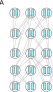
\includegraphics{figures/pedigree0}
    % 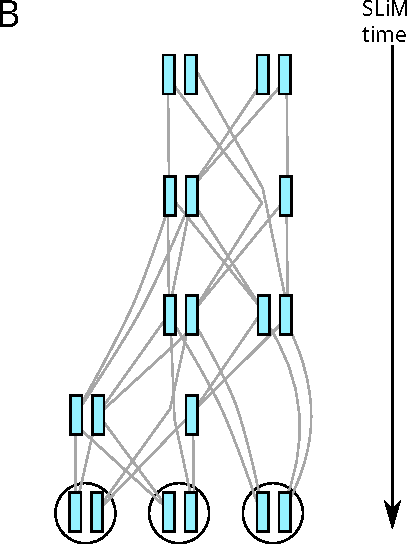
\includegraphics{figures/pedigree1}
    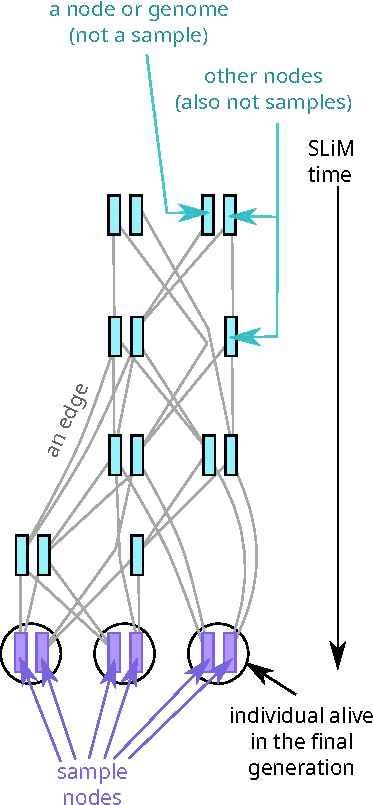
\includegraphics{figures/pedigree2}
    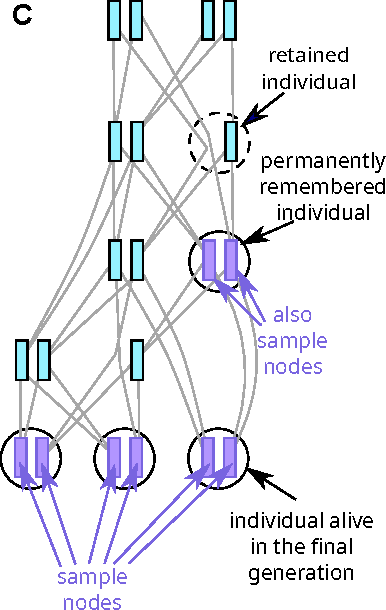
\includegraphics{figures/pedigree_remember}
\caption{
    \textbf{(A)} All relationships in a small simulation
    (three diploids over five generations).
    \textbf{(B)} Those relationships left at the end of the simulation.
    \textbf{(C)} Additional individuals may be ``remembered'' (purple)
        or ``retained'' (dotted).
    \comment{TODO: align the figures and add "B" and "C".}
}
\label{fig:indivs}
\end{figure}

\paragraph{Who is and isn't in the tree sequence:}
Suppose we have run a very small simulation with SLiM. The genetic relationships between
the various diploid individuals who were alive over the course of the simulation might
look something like Figure~\ref{fig:indivs}A. Since individuals (circles) are diploid, each contains
two genomes, which are each represented by one node (shaded rectangles).
\comment{SSG: suggest using 'genome' instead of 'chromosome' here to stay consistent with the terminology explanation above}
The edges of the tree sequence record which specific parts of the genome are inherited,
so the relationships recorded in the tree sequence are between the nodes and not the individuals directly.

In most cases, analyses will only focus on those nodes that are still alive in the final generation
of the simulation, called \textit{samples}. This renders large portions of the tree sequence irrelevant, as they
correspond to lineages that died out at some earlier point in the simulation (but see section below on
'Historical Individuals' about how to model ancient samples in a SLiM/tree sequence framework). To avoid having to
store this large quantity of unnecessary information, SLiM periodically \textit{simplifies} the tree sequence
as the simulation goes along. By default, simplification will only keep the portions of the
genetic genealogy that are required to represent the history of the current nodes
\citep{kelleher}. Additionally, it defaults to removing any node that is not a genetic
\textit{most recent common ancestor} (MRCA) of at least two daughter nodes. This removes historical
nodes that are only ``on the line to'' a sample, but do not represent a branching point
(\ie coalescent event) on the tree.

As a result of this process, the output tree sequence will look something like Figure~\ref{fig:indivs}B.
%% SSG: could move the bit in between here to the caption?
(The tree sequence also records \emph{which segments} of the genome are inherited
along each edge in the figure, but we do not attempt to depict that here).
%%
Individuals who are alive at the end of the simulation automatically have their nodes marked as
\textit{samples}, and thus their full genetic ancestry is retained. All other historical (\ie dead)
individuals (depicted as circles) have vanished, although some of their nodes remain. These nodes
have only been retained because they are required to accurately represent the
ancestry of a sample node and/or the relationships among sample nodes. Put simply,
simplification removes any nodes that have not made a genetic contribution to the sample set of nodes,
along with any associated edges.

%%%%%%%% %%%%%%%%%%%%%%
\section*{Historical individuals}
By default, only the nodes associated with individuals alive in the final generation are part of the 'sample'.
However, there are many cases where we might want to retain the complete ancestry, and other metadata, for
historical nodes. For example, we might want to model the relationship between a modern population and
one particular individual from the past.
%% SSG - another example, can cut
Or, if we are conducting simulations in parallel that share 
a common ancestry, we may need to retain certain nodes that are critical for linking diverging
tree sequences back together.
%%
The solution is to ``remember'' an individual during the course of the simulation,
using the SLiM function \verb|treeSeqRememberIndividuals()|.

\paragraph{Permanently remembering individuals}
By default, a call to \verb|treeSeqRememberIndividuals()|
will permanently remember one or more individuals,
the simulated equivalent of ancient DNA dug out of permafrost.
This means any tree sequence subsequently recorded will always contain this individual,
its nodes (now marked as samples), and its full ancestry.
The result of remembering an individual in the introductory example is pictured
in Figure~\ref{fig:indivs}C.
This is useful to, for instance, access allele frequencies and spatial locations of individuals
at a particular time in the past.

\paragraph{Retaining individuals}
\comment{SSG: I think we might need to explain in a bit more detail the kind of info associated with 'individuals' in contrast to nodes in an earlier section. For example, individuals are associated with spatial positions, two parents (in diploid case), etc. while nodes are not. The reason for 'retaining' does not seem super clear otherwise (while the case for 'remembering' is clear)}
Alternatively, you may want to only retain historical individuals as long as their nodes are still
relevant to reconstructing the genetic ancestry of the sample nodes.
This retains information that is specific to individuals as opposed to their nodes,
such as, their two parents (in diploid simulations) and their location (in spatial simulations).
This is less burdensome than remembering everyone alive, as individuals be still removed once their
nodes (which are not marked as samples) are no longer ancestral.
You can \emph{retain} individuals in this way by using
\verb|treeSeqRememberIndividuals(..., permanent=F)|.
Since a retained individual’s nodes are not considered samples,
they are subject to the standard removal 'rules' of simplification.
It is therefore possible to end up with an individual containing only one genome, as shown in the diagram.
However, as soon as both nodes of a retained individual have been lost,
the individual is deleted too.

As previously discussed, simplification will, by default, only keep nodes if they are a coalescent point
(\ie they are a MRCA or branch point) somewhere along the genome.
This can be changed by initialising tree sequence recording in SLiM using
\verb|treeSeqInitialize(retainCoalescentOnly=F)|.
SLiM will then preserve all retained individuals while they remain in the genealogy of present-day individuals,
even if their nodes are not coalescent points in a tree. These non-coalescent nodes are referred to as
unary nodes.
If you later decide to reduce the number
of samples in the tree sequence, you can do so using the tskit function simplify(),
which mirrors SLiM's version of the same procedure.
In this case, individuals that are 'retained', rather than 'remembered', will be kept only
if they are still MRCAs in the ancestry of the selected samples.
To preserve them even if their nodes are not coalescent points,
you can specify
\verb|ts.simplify(selected_samples, keep_unary_in_individuals=True)|.

\paragraph{Remembering everyone}
\comment{probably remove this}
Although not needed to reconstruct full genomic history,
it is perfectly possible to apply \verb|treeSeqRememberIndividuals()| to every individual
in every generation of a simulation (everyone who has ever lived).
If you simply mark everyone for temporary retention,
it should not increase the memory burden of your simulation much:
most individuals will be removed as the simulation progresses,
since they will not contain coalescent nodes.
However, if you use \verb|treeSeqInitialize(retainCoalescentOnly=F)|,
the number of individuals in the resulting tree sequence is likely to become very large,
and the efficiencies provided by tree sequence recording will be substantially reduced.
Indeed in this case,
retaining will be much the same as permanently remembering everyone who has ever lived.
Nevertheless, if you are willing to sacrifice enough computer memory,
either of these is (perhaps surprisingly) possible, even for medium-sized simulations.


%%%%%%%%%%%%%%%%%%%%%%%
\section{Recapitation: tying up loose ends}

\begin{figure}
\centering
    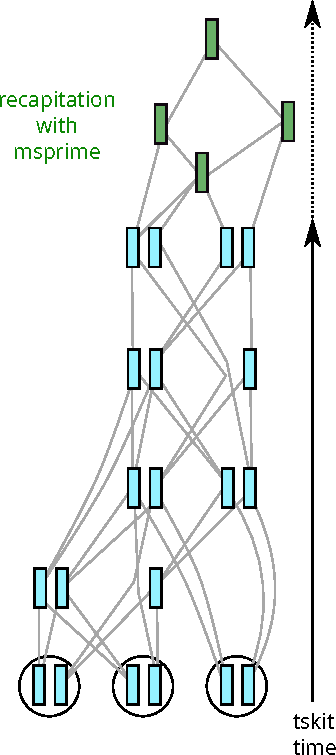
\includegraphics{figures/pedigree_recapitate}
    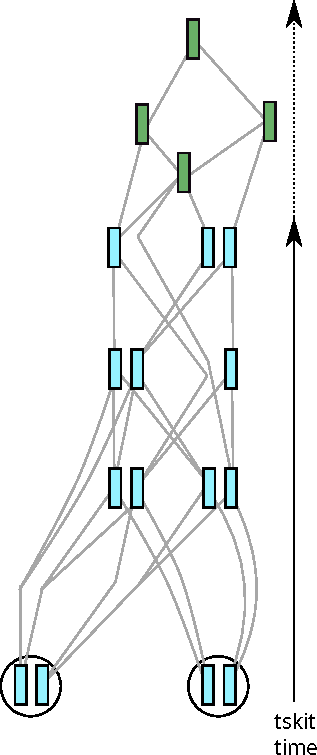
\includegraphics{figures/pedigree_simplify}
\caption{
    \textbf{(A)} Recapitation adds the green nodes 
    to the simulation of Figure~\ref{fig:indivs} by coalescent simulation.
    \textbf{(B)} The result of \emph{simplifying} the tree sequence in (A)
    down to the four sample nodes shown.
}
\label{fig:recap_simp}
\end{figure}

By default, a \slim simulation begins with all individuals identical.
This is clearly undesireable; the usual way to avoid after-effects of this
is to include a long ``burn-in'' period to generate genetic diversity.
However, this period needs to be quite long (5--15N generations),
so an attractive alternative is to initialize the simulation
with genetic diversity from a coalescent simulation.
This is what ``recapitation'' is --
except, if during the simulation we don't actually use the genotypes for anything,
it is simpler and more efficient to simply add this bit on afterwards,
only doing a coalescent simulation for those portions of the first-generation ancestors
that have not yet coalesced.
This is discussed in more detail in \citet{kelleher} and \citet{slim_manual}.
This is depicted in Figure~\ref{fig:recap_simp}A:
imagine that at some sites, some of the samples
don't share a common ancestor within the SLiMulated portion of history (shown in blue).
Recapitation starts at the \textit{top} of the genealogies,
and runs a coalescent simulation back through time
to fill out the rest of genealogical history relevant to the samples.
The green chromosomes are new ancestral nodes that have been added to the tree sequence.
If we did not do this,
then effectively we are assuming the initial population was genetically homogeneous,
and so our simulation would have less genetic variation than it should have
(since the component of variation from the initial population would be omitted).

Recapitation within a single randomly-mating population of a given size
can be done by a simple call to
pyslim.recapitate(ts, ancestral\_size=N). % TODO format
However, pyslim.recapitate is a wrapper around
msprime.sim\_ancestry, so recapitation can be done using any model simulatable by \msprime
\citep{baumdicker} --
for instance, a nonuniform genetic map --
by passing in the relevant arguments for msprime.sim\_ancestry.

We'll demonstrate recapitation with a two-population model,
since setting up an \msprime demographic model that is consistent with the SLiM simulation
requires understanding some of the details.
Recapitation happens by passing the tree sequence to the
\texttt{initial\_state} argument of \texttt{msprime.sim\_ancestry},
along with a demographic model.
The root of each uncoalesced lineage in the tree sequence is a node
that exists at a particular time and in a particular population;
these two things situate the linear within the demographic model,
so \msprime can continue following the lineages back through time.
Suppose that we've used \slim to simulate two populations, \ie with the following block:
\begin{lstlisting}{language=slim}
1 early() {
   sim.addSubpop("p1", K);
   sim.addSubpop("p2", K);
}
\end{lstlisting}
\comment{TODO provide link to or name of full slim recipe}
If the resulting tree sequence is stored in the file \texttt{migrants.trees},
then examining the populations using the shell, we see:
\begin{lstlisting}{language=bash}
> tskit populations migrants.trees
id	metadata
0	None
1	{'name': 'p1', 'slim_id': 1}
2	{'name': 'p2', 'slim_id': 2}
\end{lstlisting}
There are \emph{three} populations, but the first one is unused,
because \slim stores population \texttt{pX} as population \texttt{X}.
So, the \msprime demographic model needs to have three populations as well,
but the first population will remain unused (unless we set up migration to it).
\msprime provides a simple way to get an appropriate set-up;
\begin{lstlisting}{language=py}
demography = msprime.Demography.from_tree_sequence(ts, initial_size=100)
\end{lstlisting}
If we recapitated with this demography,
\msprime would run forever,
because there is no way for linages in one population
to coalesce with those in the other.
Suppose we wanted one-directional migration from \p1 to \p2
(so that lineages in \p2 moved back into \p1)
starting 100 generations before the start of the SLiM simulation.
To add this, then recapitate and add mutations:
\begin{lstlisting}{language=py}
demography.add_migration_rate_change(
    time=ts.metadata['SLiM']['tick'] + 100,
    rate=0.1, source="p2", dest="p1",
)
rts = pyslim.recapitate(ts, demography=demography,
            recombination_rate=1e-8)
\end{lstlisting}

The final step is likely adding neutral mutations,
again with \msprime -- see the pyslim manual.


%%%%%%%%%%%%%%%%%%%%%%%
\section{Using \msprime-generated diversity in \slim}

Simulations of large populations with selection can be costly,
especially because we might need to run a lengthy ``burn-in'' period
to get the genetic variation for selection to act on,
and because we actually need the genetic variation within \slim,
we can't add it on after the fact as in the previous section.
However, because the precise form of the burn-in may not be important, 
one strategy is to run a neutral burn-in with \msprime,
and then have selection start acting on this diversity in \slim.
This is of course not the same thing as running a burn-in with selection,
but all approaches are approximations
(for instance, the burn-in-with-selection would be started with no diversity),
and it seems to us to be in most cases a reasonable one.

A concrete scenario is as follows:
imagine we perform a lab experiment in which
we take high-diversity organisms from the wild
and subject them to selection for a few dozen generations.
Although genetic diversity in the wild is most likely not neutral,
we do not know precisely what it does look like
and a coalescent simulation would be an acceptable starting point.
The key attribute of reality we would like to approximate
is the joint distribution of allele frequencies and effect sizes.
If the alleles affect a trait under stabilizing selection,
we would expect a negative correlation between the two.
On the other hand, there would be no relationship between allele frequencies and effect sizes
if the trait we are selecting on in the lab is not under strong selection in the wild.
The precise scenario we simulate is where the trait
is not under stabilizing selection in the wild,
but we put it under selection in the lab.
To do so, we will:
\begin{enumerate}
    \item Run a coalescent simulation with msprime.
    \item Add \slim metadata to the nodes, individuals, and populations.
    \item Add \slim mutations with msprime,
        and edit the mutation metadata to assign selection coefficients.
    \item Run the \slim portion of the simulation.
    % \item Do some descriptive analysis of the results of selection.
    % \item Add neutral mutations to the tree sequence.
    % \item Do some descriptive analysis of genetic diversity along the genome.
\end{enumerate}

Concretely, we'll simulate XXX OVERVIEW OF mutation rates etc


\subsection*{Annotating tree sequence with SLiM metadata}

Suppose that the coalescent simulation has already been done,
but mutations have not been added,
producing the tree sequence \verb|ots|.
This tree sequence has genealogical information:
individuals, nodes (chromosomes), and relationships between them,
but no SLiM-specific information and no genetic diversity.
First, we add SLiM metadata to all of these things, a procedure we call ``annotating''.
\begin{listing}[H]
  \begin{minted}[fontsize=\small, linenos, bgcolor=gray!10]{python}
ots = pyslim.annotate(ots, model_type="WF", tick=1, stage="late")
  \end{minted}
\end{listing}
This \pyslim method adds default metadata to everything that needs it:
in this case, all individuals, all nodes that are part of alive individuals,
and all populations referenced by nodes.
These default values are returned by \verb|slim_default_metadata()|
(\eg all individuals are hermaphrodite, all chromosomes are autosomal).
We demonstrate how to modify this metadata by adding selection coefficients to mutations below,
but other changes (\eg assigning sexes) is similar.
For instance, top-level metadata now shows:
\begin{listing}[H]
    \begin{minted}[fontsize=\small, linenos, bgcolor=gray!10]{python}
tables.metadata
    \end{minted}
\end{listing}
\begin{pycon}
{
    'SLiM': {
        'cycle': 1, 
        'description': '', 
        'file_version': '0.8', 
        'model_type': 'WF', 
        'name': '', 
        'nucleotide_based': False, 
        'separate_sexes': False, 
        'spatial_dimensionality': '', 
        'spatial_periodicity': '', 
        'stage': 'late', 
        'tick': 1
        }
}
\end{pycon}
This metadata needs to match our planned slimulation --
particularly the \verb|model_type| (WF or nonWF) and the \verb|tick|
(which tells SLiM what value to set the tick counter to once this tree sequence is loaded).

\subsection*{Adding mutations with SLiM metadata}

Next, we will use the \verb|msprime.SLiMMutationModel| to add mutations to the tree sequence.
These will all be neutral,
so, we next modify their metadata to have selection coefficients drawn from some distribution.
We will want this to be as if we'd done it in a burn-in script in \slim:
\begin{lstlisting}{language=slim}
        initializeMutationType("m2", 0.5, "f", 0.001);
        initializeMutationRate(3e-10);
\end{lstlisting}
In other words, we would like mutations to be of type \verb|m2|,
and to assign selection coefficients to the fixed value 0.001.
% (but, of course, this is a coalescent simulation,
% so the dynamics of the mutations up until this point have been neutral).
% Note that the dominance coefficient is not stored in the tree sequence:
% it gets set in the SLiM recipe because it is a property of the mutation type,
% not of individual mutations, in SLiM.
To add SLiM mutations with \msprime, we use the built-in
\verb|SLiMMutationModel|:
\begin{listing}[H]
    \begin{minted}[fontsize=\small, linenos, bgcolor=gray!10]{python}
mut_model = msprime.SLiMMutationModel(type=2)
ots = msprime.sim_mutations(ots, rate=3e-8, model=mut_model)
  \end{minted}
\end{listing}
The \verb|type=2| argument to \verb|msprime.SLiMMutationModel|
means the mutations will be of type ``m2'' in SLiM
(and, so you must initialize that mutation type in the SLiM recipe).
Those mutations have selection coefficient 0
(as they should, since in this portion of history they've been neutral);
but now we want to change that.
Doing this follows a general pattern for editing a tree sequence:
make a copy of the underlying \emph{tables};
clear the relevant table;
then write back in the information, modifying as desired.
\begin{listing}[H]
    \begin{minted}[fontsize=\small, linenos, bgcolor=gray!10]{python}
tables = ots.dump_tables()
tables.mutations.clear()
for m in ots.mutations():
  md_list = m.metadata["mutation_list"]
  for md in md_list:
    md["selection_coeff"] = 0.001
  tables.mutations.append(
      m.replace(metadata={"mutation_list": md_list})
  )
  \end{minted}
\end{listing}
We edit the \emph{tables} because a tree sequence is (for efficiency reasons) immutable.
For a more complex example that draws coefficients randomly (and so requires more bookkeeping),
see the pyslim documentation.
\comment{Do we need this? I think so, sadly...}
To understand this code we need to understand \slim's mutation model --
\emph{warning:} fiddly, nitpicky details to follow.
In \slim, each genome at each has a \emph{collection} of abstract ``mutations''.
(In most cases, there will be zero or one mutation at a given position,
but there can be more.)
Mutations thus do not necessarily represent single-nucleotide changes.
However, the mutation model in \tskit is different, requiring that each mutation
\emph{replace} the previous allele with a new allele (rather than allowing stacking, like \slim).
So, a single mutation in the tree sequence corresponds to a collection of \slim mutations,
which we record in two ways.
First, the \verb|derived_state| of the mutation is a comma-separated list of SLiM mutation IDs.
Second, the mutation's metadata has one entry: \verb|"mutation_list"|,
which is a list of metadata entries.
For instance, here is a muutation as stored in the tree sequence
that was the result of a (rare) double hit:
\begin{listing}
    \begin{minted}[fontsize=\small, linenos, bgcolor=gray!10]{python}
Mutation(id=295, site=180, node=43931, derived_state='193,194',
    parent=294, time=8.74,
    metadata={'mutation_list': [
        {'mutation_type': 2, 'selection_coeff': 0.001, 'subpopulation': -1, 'slim_time': -559, 'nucleotide': -1},
        {'mutation_type': 2, 'selection_coeff': 0.001, 'subpopulation': -1, 'slim_time': -7, 'nucleotide': -1}
    ]})
    \end{minted}
\end{listing}
This mutation occurred
above node 43931 at a position on the genome we could obtain by looking at site 180.
Genomes that inherit this mutation carry at this site two \slim mutations with IDs 193 and 194;
these mutations are labeled with \slim time -559 and -7 generations, respectively.
Since the first of the two occurred longer ago (a larger negative \slim time),
we can infer that the mutation with \slim ID 194 occurred on the background
of the mutation with \slim ID 193.
% We can confirm this by looking at the ``parent'' mutation whose ID is 294,
% and has derived state simply 193.
Sharp-eyed readers will note that the ``time'' of the mutation given by the tree sequence
(8.74 generations ago) does not match the ``\slim time'' recorded in metadata
(-7 generations in the future);
in general this conversion is ``rounded and maybe off by one, depending on the model type''.
For a detailed discussion of conversion between time in the tree sequence
and time in the SLiM model, see the pyslim documentation.


\subsection*{Loading into SLiM}

Now, we can move onto the SLiM recipe
that loads the edited tree sequence back in.
This simply continues selected mutations as before
(with mutation rate \num{3e-10} per bp per generation and the same distribution of fitness effects).
The population size is determined by the number of individuals
that were read in from the tree sequence.
We need to make sure that the genome lengths match,
so we provide that as a constant \verb|L|, that will be provided at run time.
To facilitate later analysis,
we’ll also ``Remember'' the individuals present at the start of the simulation,
so that they will remain in the tree sequence.
Supposing we've dumped the edited tree sequence as ``init.trees'':
\begin{lstlisting}[language=slim]
initialize()
{
    // must define L
    initializeSLiMModelType("WF");
    initializeTreeSeq();
    initializeMutationRate(3e-10);
    initializeMutationType("m1", 0.5, "f", 0.0);
    initializeMutationType("m2", 0.5, "e", 0.01);
    initializeGenomicElementType("g1", m2, 1.0);
    initializeGenomicElement(g1, 0, L-1);
    initializeRecombinationRate(1e-8);
}

1 late() { 
    sim.readFromPopulationFile("init.trees");
    sim.treeSeqRememberIndividuals(p0.individuals);
}

100 late() {
    catn("Done.");
    sim.treeSeqOutput("vignette_annotated.trees");
    sim.simulationFinished();
}
\end{lstlisting}

Note that the simulation only has selected mutations (of type \verb|m2|),
but as we will add in type \verb|m1| mutations later,
we have declared them in the recipe as a placeholder.
We could run this on the command line as \verb|slim -d L=100000000 reload_annotated.slim|.


\subsection*{Overlaying neutral mutations}

In real data, of course, we do not get to observe selection coefficients.
We have not added in neutral mutations until this point for efficiency - they are just bookkeeping,
and do not affect the course of the simulation in any way.
For this reason, we can add them in after the fact,
in a way that is exactly equivalent to having kept track of them as we went along.

Recall that out of an overall mutation rate of \num{3e-8},
we wanted 99\% of the mutations to be neutral.
So, we will now add mutations at rate $0.99 \times 3 \times10^{-8}$.
The code is nearly the same as before,
except for setting the ``type'' to 1
(so that neutral mutations would show up in SLiM as \verb|m1|),
and we have asked these mutations to have SLiM mutation IDs beginning at the ID where the previous mutations left off.
(This would be important were we to read this tree sequence back in to SLiM;
mutation IDs must be unique.)
And, importantly, we’ve added \verb|keep=True| so that existing mutations are not discarded.
\begin{listing}[H]
    \begin{minted}[fontsize=\small, linenos, bgcolor=gray!10]{python}
next_id = pyslim.next_slim_mutation_id(ts)
neutral_mut_model = msprime.SLiMMutationModel(type=1, next_id=next_id)
mts = msprime.sim_mutations(
                ts,
                rate=0.99 * 3e-8,
                model=neutral_mut_model,
                keep=True)
    \end{minted}
\end{listing}

% \begin{pycon}
% The tree sequence now has 443071 mutations, at 431899 distinct sites.
% \end{pycon}
% 
% Now, we have a lot more mutations! And some of the sites have more than one mutation:
% 
% \begin{listing}[H]
%     \begin{minted}[fontsize=\small, linenos, bgcolor=gray!10]{python}
% num_alleles = np.array([len(s.mutations) for s in mts.sites()])
% for k in range(1, max(num_alleles)+1):
%   print(f"There are {sum(num_alleles == k)} sites with {k} distinct alleles.")
%     \end{minted}
% \end{listing}
% \begin{pycon}
% There are 420920 sites with 1 distinct alleles.
% There are 10790 sites with 2 distinct alleles.
% There are 185 sites with 3 distinct alleles.
% There are 4 sites with 4 distinct alleles.
% \end{pycon}

\subsection{VCF output}

It might seem irrelevant to use the \verb|SLiMMutationModel| again
if we don't plan to read the resulting tree sequence back into \slim.
However, it's important: if we'd omitted the \verb|model| argument
(thus using the default Jukes-Cantor model),
we probably would have got an error:
``\textit{Existing allele(s) incompatible with mutation model alphabet.}''
This error occurs when the Jukes-Cantor (which only knows about alleles A, C, G, and T)
encounters an allele it doesn't recognize
(such as a comma-separated list of integers, as produced by the \slim mutation model).
Similar problems occur if you output the tree sequence as a VCF,
which will be deeply confused by these alleles.
\pyslim includes tools to make this output easy:
\verb|generate_nucleotides| to add nucleotides to non-nucleotide models,
and then \verb|convert_alleles| to replace the comma-separated-list-of-integer alleles
with the underlying nucleotide alleles.
So, to output to VCF we'd do:
\begin{listing}[H]
    \begin{minted}[fontsize=\small, linenos, bgcolor=gray!10]{python}
nts = pyslim.generate_nucleotides(ts)
nts = pyslim.convert_alleles(ts)
with open('nucs.vcf', 'w') as f:
    nts.write_vcf(f)
    \end{minted}
\end{listing}
This code will generate independent, uniformly chosen nucleotides
for each ancestral state and derived states for each mutation
from the Jukes-Cantor model.


%%%%%%%%%%%%%%%%%%%%%%%%%%%%%%
\section*{Parallelizing forward-in-time simulations of multiple species}
\comment{stitch together with the previous section: there was msp+slim, here is slim+slim}
Any two branches stemming from the same node in a species tree are independent from each other and
thus can be simulated in parallel (assuming no migration between the species).
For example, in the phylogeny depicted in Figure~\ref{fig:phylo},
branches of the same color can be simulated in parallel.
To do so, we will need to
(i) simulate the history of each branch and
(ii) join the resulting simulations together onto one multi-species history.

 \begin{figure}[h!]
 \centering
  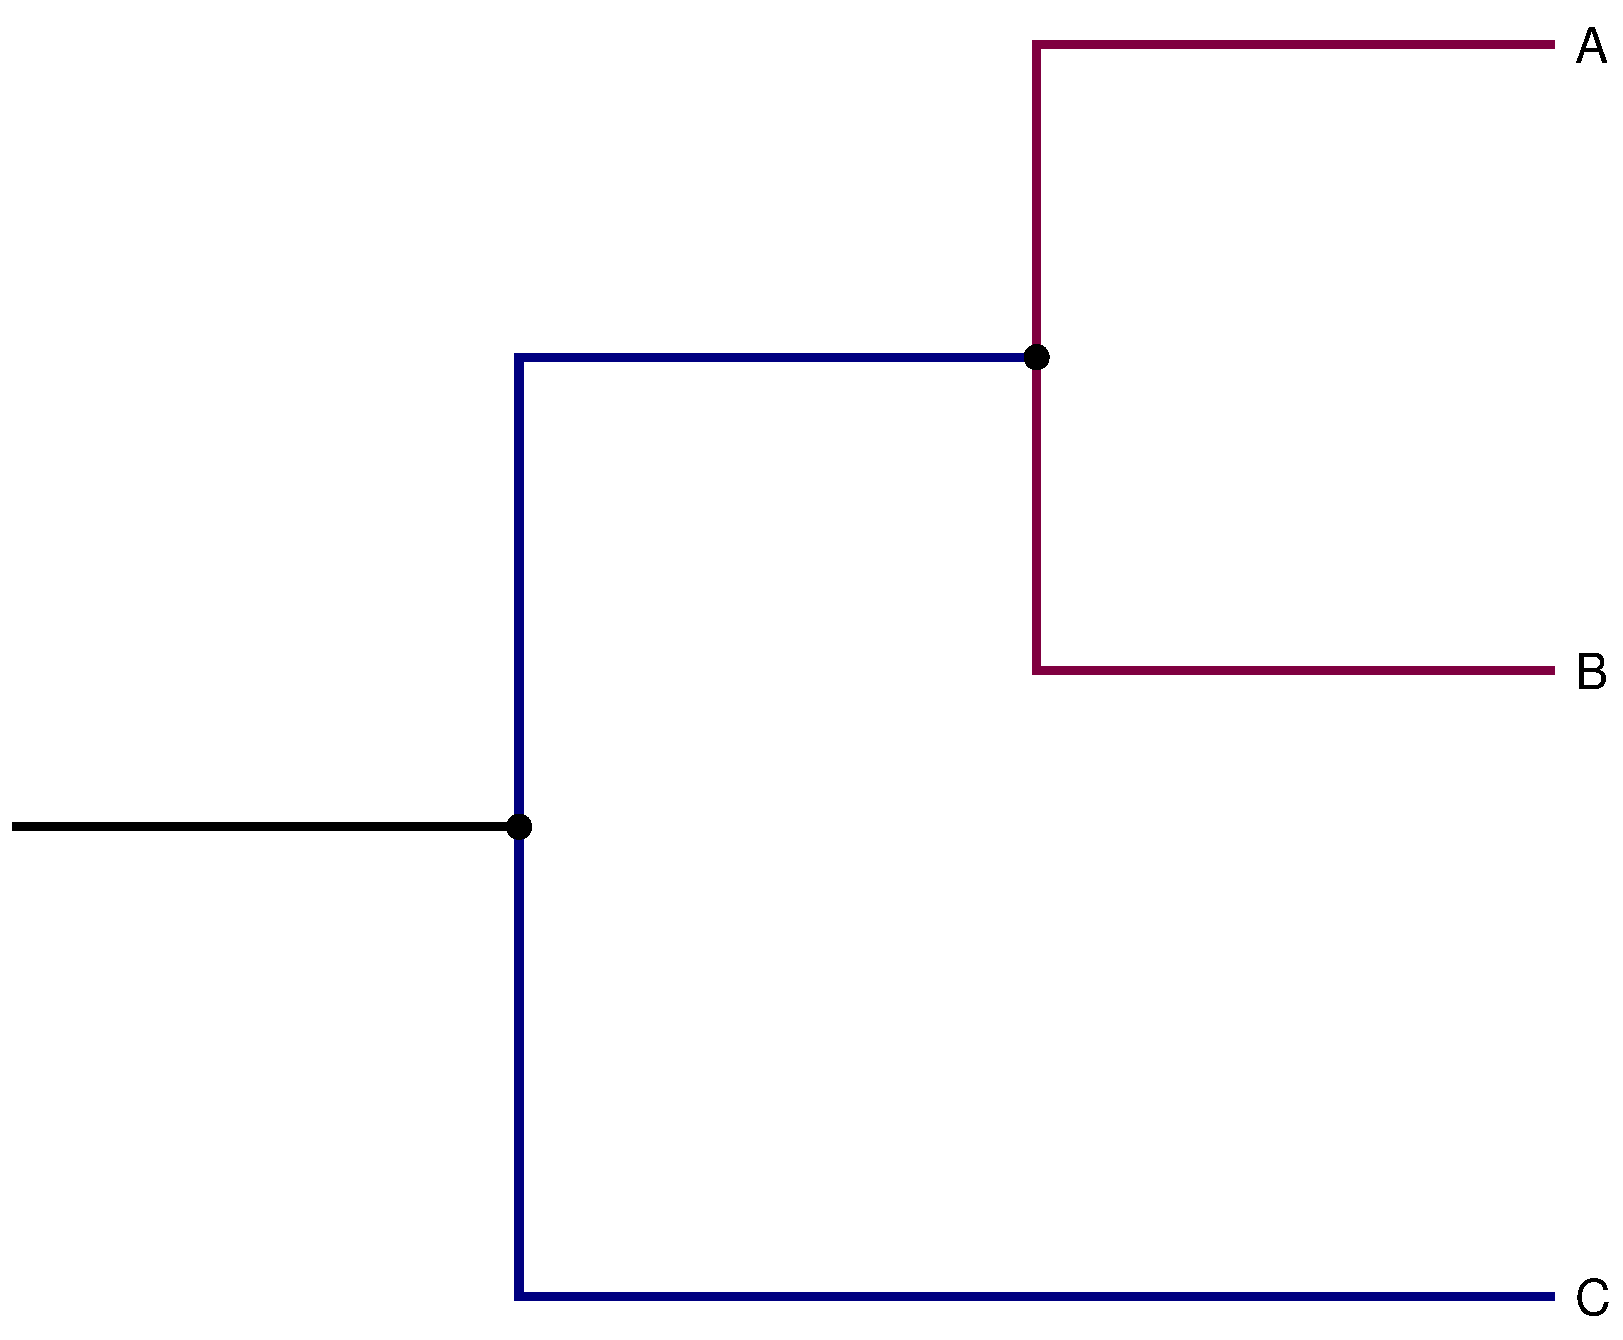
\includegraphics[width=0.5\textwidth]{./code/parallelizing_phylogeny/phylo.pdf}
  \caption{Example of phylogeny we might want to simulate. Note how branches with the same color can be simulated in parallel when there is no migration.}
  \label{fig:phylo}
 \end{figure}

\subsection{Parallel simulation of branches}

First, we need to write a \slim script that will be used for simulating the history of each branch in our phylogeny.
We will perform a simple simulation,
in which each branch can have a different (but fixed) population size and length (number of ticks).
Also, we will allow deleterious mutations to happen across the entire chromosome at a fixed rate.
See the code below (Listing~\ref{lst:slim-example}).

\begin{listing}[H]
  \inputminted[fontsize=\small, linenos, bgcolor=gray!10]{javascript}{./code/parallelizing_phylogeny/simulate_branch.slim}
  \caption{Simple \slim script to simulate a constant size population that can be started from an existing tree sequence.}
  \label{lst:slim-example}
\end{listing}

For each branch, the presence or absence of \verb|infile| tells \slim whether a previous branch exists or not.
If so, \slim will read the previous tree sequence and change the population size accordingly.
Note that when you read a tree sequence into \slim,
the tick counter will be updated with the time encoded in the tree sequence,
so we need to set the end of the simulation as the length of the branch (\verb|num_gens|)
plus the current “time” at the end of the loaded tree sequence.
At the end of the simulation, we call \verb|sim.treeSeqRememberIndividuals| right before saving the resulting tree sequence.
This is necessary because we need to ensure the individuals in the final generation are never dropped
from the tree sequence in future runs of \slim which are started from the output of the simulation,
as they will later be used to glue the tree sequences together.

The example phylogeny we will simulate is encoded in the table below (Table~\ref{tab:phylo}).

\begin{table}[H]
  \centering
  \caption{Parameters of the phylogeny that will be simulated.}
  \label{tab:phylo}
    \begin{tabular}{llll}
      \bfseries Child & \bfseries Parent & \bfseries Population size & \bfseries Edge length \\
      \hline
      \csvreader[head to column names]{./code/parallelizing_phylogeny/phylo.csv}{}%
        {\child & \parent & \popsize & \edgelen\\}
    \end{tabular}
\end{table}


%%%%%%%%%%%%%%%%%%%%%%%%%
\section*{Networks of simulations: within-host dynamics}

As a final example, we'll look at a situation that is very different to the usual \slim simulation.
Pathogens often have very large population (census) sizes,
but spread out across many host individuals with between-host dynamics
that are daunting to simulate.
However, the dynamics \emph{within} a host are closer to a standard \slim simulation,
which makes this a good target for parallelization:
the dynamics within each host is a single job;
each job may create new jobs (new infections)
or interact with other jobs (co-infection).
Maintaining a tree sequence across these runs is conceptually similar
to the previous section, but has additional difficulties.

To do this, we have a \slim script that describes dynamics within a single host.
This script begins by loading in a tree sequence
that contains the pathogen individual(s) that initiated the infection and their history,
and at some later point writes out a tree sequence containing the individual(s) that infect other host(s)
and their history.
Then, we use job scheduling software to organize the simulation runs.
There are thus two important steps to describe:
first, how individuals are ``transmitted'' from one simulation to the next;
and second, how we combine the resulting tree sequences.
There are various ways to set this up; we describe one method that makes bookkeeping
less daunting.

A first attempt at transmission between hosts would simply save the state of the population
at the desired time, and then the \slim run describing the next host
would start from this state by selecting a few individuals as those that were transmitted.
However, this can easily lead to contradictions: for instance,
if one host infects two other hosts,
then a single individual who was present in the first host simulation
might die at different times in the simulation runs of the two subsequent hosts.
So, coordination is required.
\slim can write out arbitrary information to text files,
but the most convenient place to record auxilliary information that goes along with a given tree sequence
is usually in the ``top-level metadata'',
which is visible in both \slim and python as a dictionary
(in python, as \verb|ts.metadata|).
So, whenever a new host is to be infected,
we select some ``founder'' individuals to start the infection;
Remember these founders and then kill them;
and then write down their IDs in the metadata
(under a key which identifies the host they're going on to infect).
Then for each subsequent host
we use a python script to post-process the resulting tree sequence
so that the founder individuals will be ``alive'' (and no others)
when the tree sequence is loaded into \slim.

The next task is to combine the partially-overlapping histories of different hosts.
As in the previous section, we use \verb|union| to do this;
however, we need to work a little harder
to identify the portions of history that are shared between two tree sequences.
To do this, we need to
(a) find the founders that are present in both tree sequences,
and (b) identify all nodes that are ancestral to these founders.
The first step is easily done by consulting metadata.
Here is code that identifies all ancestors in the tree sequence
of a given set of nodes:
\begin{lstlisting}{language=py}
def ancestors(ts, nodes):
    """
    Returns the list of nodes reachable from `nodes` by following
    child->parent relationships in the edge table.
    """
    out = np.zeros(ts.num_nodes, dtype='int')
    out[nodes] = 1
    x = out.copy()
    A = scipy.sparse.coo_array(
            (
                np.ones(ts.num_edges, dtype='int'),
                (ts.edges_parent, ts.edges_child)
            ), dtype='int', shape=(ts.num_nodes, ts.num_nodes)
    )
    while np.sum(x) > 0:
        x = A @ x
        out += x
    return np.where(out > 0)[0]
\end{lstlisting}
With this in hand, we can use \verb|union|
as in the prvious section.



%%%%%%%%%%%%%%%%%%%%%%%%%
\section*{Author contributions}

%%%%%%%%%%%%%%
\newpage
\appendix

\comment{STUFF WE MAYBE DON'T WANT: moved here from above:}

\comment{Remove ILS thing and just add a paragraph citing Rodrigues et al and saying why this would be faster and would split the memory requirements across a bunch of processes.}

\section{Recapitation}


Doing this is as simple as:

\begin{lstlisting}{language=slim}
orig_ts = tskit.load("example_sim.trees")
rts = pyslim.recapitate(orig_ts,
            recombination_rate=1e-8,
            ancestral_Ne=200, random_seed=5)
\end{lstlisting}
The warning is harmless; it is reminding us to think about generation time
when recapitating a nonWF simulation (a topic we'll deal with later).

We can check that this worked as expected, by verifying that after recapitation
all trees have only one root:
\begin{lstlisting}{language=slim}
orig_max_roots = max(t.num_roots for t in orig_ts.trees())
recap_max_roots = max(t.num_roots for t in rts.trees())
print(f"Maximum number of roots before recapitation: {orig_max_roots}\n"
      f"After recapitation: {recap_max_roots}")
\end{lstlisting}

The `.recapitate` method
is just a thin wrapper around `msprime.sim\_ancestry`,
and you need to set up demography explicitly - for instance, in the example above
we've simulated from an ancestral population of ``Ne=200`` diploids.
If you have more than one population,
you must set migration rates or else coalescence will never happen.
% (see [](sec_recapitate_with_migration) for an example, and {func}`.recapitate` for more).

(TODO: mention about how to recapitate with a nonuniform map, as in the docs?)


\section{Simplification}


Probably, your simulations have produced many more fictitious genomes
than you will be lucky enough to have in real life,
so at some point you may want to reduce your dataset to a realistic sample size.
We can get rid of unneeded samples and any extra information from them by using
an operation called *simplification* (this is the same basic approach that SLiM
implements under the hood when outputting a tree sequence).

Depicted in Figure~\ref{fig:recap_simp}B is the result of applying an explicit call to
simplify to our example tree sequence.
In the call we asked to keep only 4
genomes (contained in 2 of the individuals in the current generation). This has
substantially simplified the tree sequence, because only information relevant to the
genealogies of the 4 sample nodes has been kept. (Precisely, simplification retains only
nodes of the tree sequence that are branching points of some marginal genealogy -- see
CITE % [Kelleher et al 2018](https://doi.org/10.1371/journal.pcbi.1006581) for details.)
While simplification sounds very appealing - it makes things simpler after all -
it is often not necessary in practice, because tree sequences are very compact,
and many operations with them are quite fast.
(It will, however, speed up many operations, so if you plan to do a large number of simulations,
your workflow could benefit from early simplification.)
So, you should probably not make simplification a standard step in your workflow,
only using it if necessary.

It is important that simplification - if it happens at all -
either (a) comes after recapitation, or (b) is done with the
``keep\_input\_roots=True`` option.
This is because simplification removes some of the
ancestral genomes in the first generation,
which are necessary for recapitation,
unless it is asked to "keep the input roots".
If we simplify without this option before recapitating,
some of the first-generation blue chromosomes in the figure on the right
would not be present, so the coalescent simulation would start from a more recent point in time
than it really should.
As an extreme example, suppose our SLiM simulation has a single diploid who has reproduced
by clonal reproduction for 1,000 generations,
so that the final tree sequence is just two vertical lines of descent going back
to the two chromosomes in the initial individual alive 1,000 generations ago.
Recapitation would produce a shared history for these two chromosomes,
that would coalesce some time longer ago than 1,000 generations.
However, if we simplified first, then those two branches going back 1,000 generations would be removed,
since they don't convey any information about the shape of the tree;
and so recapitation might produce a common ancestor more recently than 1,000 generations,
which would be inconsistent with the SLiM simulation.

After recapitation,
simplification to the history of 100 individuals alive today
can be done with the {meth}`tskit.TreeSequence.simplify` method:
\begin{lstlisting}{language=slim}
import numpy as np
rng = np.random.default_rng(seed=3)
alive_inds = pyslim.individuals_alive_at(rts, 0)
keep_indivs = rng.choice(alive_inds, 100, replace=False)
keep_nodes = []
for i in keep_indivs:
  keep_nodes.extend(rts.individual(i).nodes)

sts = rts.simplify(keep_nodes, keep_input_roots=True)
\end{lstlisting}

Note that you must pass simplify a list of \textit{node IDs}, not individual IDs.
Here, we used the `.individuals\_alive\_at` method to obtain the list
of individuals alive today.
Also note that there are *still* more than 100 individuals remaining - 15 non-sample individuals
have not been simplified away,
because they have nodes that are required to describe the genealogies of the samples.
(Since this is a non-Wright-Fisher simulation,
parents and children can be both alive at the same time in the final generation.)



\section{Adding neutral mutations to a SLiM simulation}

% ```{figure} _static/pedigree_mutate.png

If you have recorded a tree sequence in SLiM, likely you have not included any neutral mutations,
since it is much more efficient to simply add these on afterwards.
To add these (in a completely equivalent way to having included them during the simulation),
you can use the `msprime.sim\_mutations` function, which returns a new tree sequence with additional mutations.
Continuing with the cartoons from above, these are added to each branch of the tree sequence
at the rate per unit time that you request.
We'll add these using the {class}`msprime.SLiMMutationModel`, so that the file can be read back into SLiM,
but any of the other mutation models in msprime could be used.
This works as follows:
\begin{lstlisting}{language=slim}
next_id = pyslim.next_slim_mutation_id(sts)
ts = msprime.sim_mutations(
           sts,
           rate=1e-8,
           model=msprime.SLiMMutationModel(type=0, next_id=next_id),
           keep=True,
)
\end{lstlisting}


What's going on here? Let's step through the code.

\begin{enumerate}
    \item The mutation ``rate = 1e-8``, which adds mutations at a rate of $10^{-8}$ per bp.
    Unlike previous versions of msprime, this adds mutations using a discrete-sites model,
    i.e., only at integer locations (like SLiM).

\item We're passing ``type=0`` to the mutation model.
    This is because SLiM mutations need a "mutation type",
    and it makes the most sense if we add a type that was unused in the simulation.
    In this example we don't have any existing mutation types, so we can safely use ``type=0``.

\item We also add ``keep = True``, to keep any existing mutations.
    In this example there aren't any, so this isn't strictly necessary,
    but this is a good default.

\item If there are existing SLiM mutations on the tree sequence we need to
    make sure any newly added mutations have distinct SLiM IDs,
    so we use `.next\_slim\_mutation\_id` to figure out
    what the next available ID is, and pass it in.

\end{enumerate}

TODO: writing out to VCF



\end{document}
